\documentclass[11pt,letterpaper]{article}
\usepackage{style}

%% ------- INICIA DOCUMENTO ------
\begin{document}
\begin{titlepage}
\begin{center}
\begin{LARGE}
INSTITUTO POLITÉCNICO NACIONAL\\
\vspace*{0.15in}
ESCUELA SUPERIOR DE CÓMPUTO\\
\end{LARGE}
\vspace*{1.0in}
\begin{Large}
%% NOMBRE DE LA PRÁCTICA O EXAMEN
\textbf{TÉCNICAS DE CRUZA 1} \\  
\end{Large}
\vspace*{0.2in}
\begin{large}
\textit{Práctica 6}\\
\end{large}
\vspace*{1.0in}
\begin{large}
%% INTEGRANTES	
Dominguez de la Rosa Bryan\\
\vspace*{2.0in}
GRUPO 3CM5\\
\vspace*{0.2in}
Profesor: Morales Güitron Sandra Luz\\
\vspace*{1.5in}
\today
\vspace*{0.3in}
\end{large}
\rule{150mm}{0.1mm}\\

\end{center}
\end{titlepage}

%% --------- COMIENZA EL DESARROLLO DEL DOCUMENTO --------

\section*{Introducción}
En esta práctica se utiliza la librería xlib de C en Linux para graficar un histograma lineal, en el cual cada punto representa el valor de un arreglo de números enteros.

\subsection*{Histrograma}
En estadística, un histograma es una representación gráfica de una variable en forma de barras, donde la superficie de cada barra es proporcional a la frecuencia de los valores representados. Sirven para obtener una "primera vista" general, o panorama, de la distribución de la población, o de la muestra, respecto a una característica, cuantitativa y continua (como la longitud o el peso).\\

\subsection*{Libreria Xlib (Linux)}
Xlib es una biblioteca que reúne un conjunto de funciones y macros realizadas en el lenguaje de programación C y utilizadas por un cliente para hacer de interfaz con el servidor gráfico de X Windows System.  En resumen, es una interfaz de programación de bajo nivel para X11. Xlib está basada en la filosofía de eventos (o mensajes). La biblioteca apareció alrededor del 1985. Algunas aplicaciones utilizan directamente Xlib, sin embargo es muy común que se utilicen bibliotecas que a la vez la utilizan, entre ellas se encuentran: X Toolkit Intrinsics (Xt), Xaw, XView, Motif, GTK+, Qt (versión para X11), Tk.\\


Proporcionan a una aplicación la posibilidad de: abrir una presentación X, crear ventanas y escribir en ellas, recuperar eventos y cerrar la presentación. Casi todas las funciones se ejecutan de forma asíncrona y son peticiones enviadas a un buffer de salida. Para el trabajo en modo síncrono se requiere de Xsync tras la función de Xlib que se quiere ejecutar en modo síncrono. 

\section*{Contenido}

Para instalar la libreria Xlib se utiliza el siguiente comando:\\
\begin{center}
	\textbf{sudo apt-get install libx11-dev}
\end{center}

Una vez instalada la librería, se desarrollo el programa. El primer paso fue generar un arreglo de números enteros, en este caso con valor fijo de 10 elementos; el arreglo debe ser llenado de números aleatorios para probar el funcionamiento con diversos valores y observar como el histograma responde a los cambios de valor.\\

Una vez teniendo el arreglo de números listo, se itera en él para obtener el valor de cada elemento y trasladarlo a un pixel de la ventana de gráficos donde se mostrará el histograma. \\

Los archivos que se tienen para la práctica son los siguientes:

Para compilar, se ejecuta el comando \textbf{make}, el cual tiene las siguientes líneas:\\
\textbf{make:\\
	gcc gfx.c -c\\
	g++ histogram.cpp -std=c++11 -c\\
	g++ gfx.o histogram.o -o histogram -lX11\\
}
	
Una vez compilado el código, pasamos a la ejecución, para lo cuál usamos el comando  \textbf{./histogram}

Algunos ejemplos de la ejecución de la práctica se muestran a continuación:\\

Ejemplo con el arreglo $\left[28,49,49,29,15,43,18,37,44,24  \right]$

\begin{figure}[H]
	\centering
	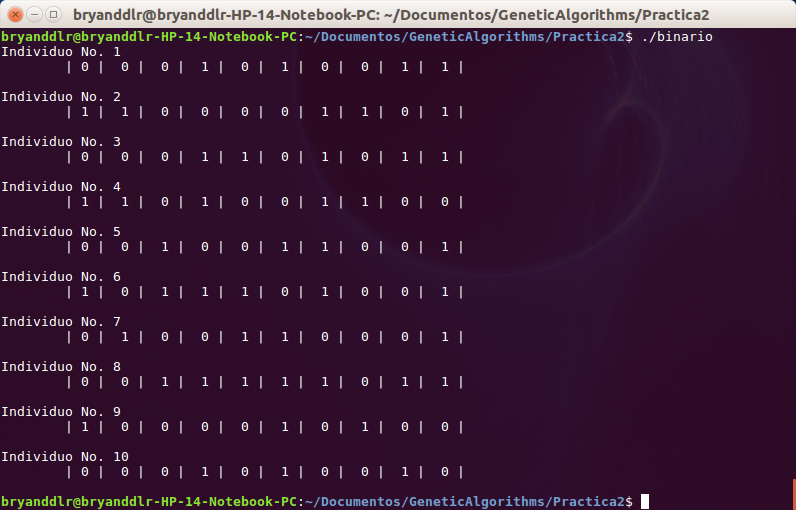
\includegraphics[scale = 0.3]{images/ej1}
\end{figure}

Ejemplo con el arreglo $\left[18,27,42,18,31,25,14,6,8,5 \right]$
\begin{figure}[H]
	\centering
	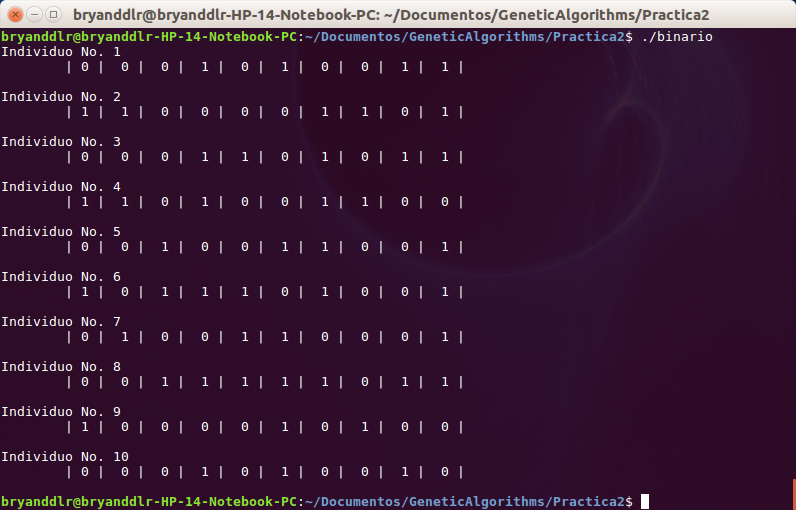
\includegraphics[scale = 0.3]{images/ej1}
\end{figure}

Ejemplo con el arreglo $\left[26,29,35,28,43,28,42,24,247 \right]$
\begin{figure}[H]
	\centering
	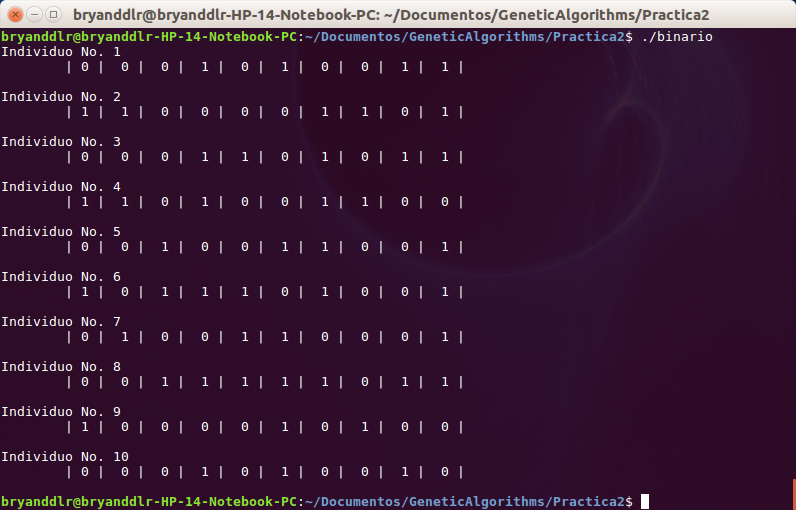
\includegraphics[scale = 0.3]{images/ej1}
\end{figure}

\section*{Conclusión}
Un histograma es una herramienta que permite visualizar estadísticas de una manera gráfica, lo cual facilita la interpretación de resultados en la ejecución de un algoritmo genético, ya que permitirá observar la evolución de los individuos en diversas generaciones, y con eso tener conclusiones acerca de que tan eficiente es nuestro algoritmo.


\end{document}
